\documentclass[journal]{IEEEtran}
\usepackage{comment}
\usepackage{multirow}
\usepackage{amsmath, amsfonts, amssymb, pifont}
\usepackage{booktabs}
\usepackage{rotating}
\usepackage{array}
\usepackage[caption=false,font=normalsize,labelfont=sf,textfont=sf]{subfig}
\usepackage{textcomp}
\usepackage{stfloats}
\usepackage{url}
\usepackage{verbatim}
\usepackage{graphicx}
\usepackage{cite}
%\usepackage[para]{footmisc}
\newcolumntype{P}[2]{%
  >{\begin{turn}{#1}\begin{minipage}{#2}\footnotesize\raggedright\hspace{1pt}}c%
  <{\end{minipage}\end{turn}}%
}
%\usepackage{tablefootnote}
\usepackage{xcolor}
\usepackage{colortbl}
%\usepackage{longtable}
\usepackage{circledsteps}
\usepackage{diagbox}
\usepackage[ruled,linesnumbered]{algorithm2e}
\usepackage{tcolorbox}
\usepackage[T1]{fontenc}
\usepackage[hidelinks]{hyperref}
\hyphenation{op-tical net-works semi-conduc-tor IEEE-Xplore}

\definecolor{Employer}{HTML}{18AFCC}
\definecolor{Platform}{HTML}{5F9099}
\definecolor{Worker}{HTML}{CC1865}

\newcommand{\cmark}{\ding{51}}
\newcommand{\xmark}{\ding{55}}

\begin{document}

\title{Appendix}

\maketitle
This appendix supplements the paper titled \textbf{Towards Open Federated Learning Platforms: Survey and Vision from Technical and Legal Perspectives}. Due to the page limitations of the journal publication, we have condensed the original manuscript and relocated some content to here.
This appendix is organized as follows: 
\begin{itemize}
    \item In \ddag\ref{apdx:related}, we present the related concepts of this survey and point out their differences.
    
    \item \ddag\ref{apdx:filter} lists our recommended filter conditions for query-based FL, along with the reasons behind each recommendation.
    
    \item In \ddag\ref{apdx:preferences}, we provide our preferences for choosing licenses in the context of model reusing, and we discuss copyright concerns related to reused results.
    
    \item In \ddag\ref{apdx:reusing}, we present our findings and discuss the relationship between model reusing and model licenses.
    
    \item \ddag\ref{apdx:how2protect} further discusses the model protection challenge, which plays an important role in advocating open FL platforms.
    
    \item \ddag\ref{apdx:decentral}, we briefly discuss some parallel works from Web3-based field and explore the opportunities for decentralization and monetization in contract-based FL.
\end{itemize}

\section{Related Topics} %%%%%%%%%%%%%%%%%%%%%%%%%%%%%%%%%%%%%%%%%
\label{apdx:related}
As summarized in TABLE~\ref{table:surveys}, most surveys extensively discuss the challenges of efficiency, heterogeneity, privacy in FL systems design, while the surveys from blockchain fields offer the most comprehensive review.
However, except for a few blockchain-based FL studies, most of the listed surveys just present the same story from slightly different angles and backgrounds, i.e., a server sets the model training task and delegates it to data holders to complete. 
This \textit{server-dominated} cooperation framework is a narrow implementation of the FL systems.
Therefore, this survey aims to fill the gap by investigating and surveying the associated tenchnologies that support more open and inclusive cooperation frameworks in FL systems, where all entities, whether they own the data or not, can benefit from it. 
%The challenges investigated in our survey are not listed in the TABLE~\ref{table:surveys}, and to the best of our knowledge, this is the first survey that focuses on the \textbf{cooperation frameworks} of FL.

\begin{table*}[t]
    \centering
    \footnotesize
    \caption{Summary of existing FL surveys. SYS denotes FL Systems Design, APP denotes FL Applications, SDC denotes Server-Dominated Cooperation frameworks.
    \cmark: elaborated, \xmark: not elaborated.}
    \label{table:surveys}
    \begin{tabular}{|l|l|lllll|lll|}
    \hline
                       & \multicolumn{1}{c|}{} & \multicolumn{5}{c|}{Challenges}                                                                            & \multicolumn{3}{c|}{Contents}                            \\ \hline
                       Scenarios/Tasks &           FL Surveys            & \multicolumn{1}{l|}{Efficiency} & \multicolumn{1}{l|}{Heterogeneity} & \multicolumn{1}{l|}{Privacy} & \multicolumn{1}{l|}{Incentive} & Decentralize & \multicolumn{1}{l|}{SYS} & \multicolumn{1}{l|}{APP} & SDC \\ \hline
    \multirow{14}{*}{General} &      Yang \textit{et al.}~\cite{yang2019federated}         & \multicolumn{1}{c|}{ \cmark } & \multicolumn{1}{c|}{\cmark} & \multicolumn{1}{c|}{\cmark} & \multicolumn{1}{c|}{\cmark} & \multicolumn{1}{c|}{\cmark}  & \multicolumn{1}{c|}{\cmark} & \multicolumn{1}{c|}{\cmark} & \multicolumn{1}{c|}{\cmark}  \\ \cline{2-10}              
                        &   Li \textit{et al.} 2020~\cite{li2020federated}                    & \multicolumn{1}{c|}{\cmark} & \multicolumn{1}{c|}{\cmark} & \multicolumn{1}{c|}{\cmark} & \multicolumn{1}{c|}{\xmark} & \multicolumn{1}{c|}{\cmark} & \multicolumn{1}{c|}{\cmark} & \multicolumn{1}{c|}{\cmark} & \multicolumn{1}{c|}{\cmark} \\ \cline{2-10} 
                        & Zhang \textit{et al.} 2021~\cite{zhang2021survey} & \multicolumn{1}{c|}{\cmark} & \multicolumn{1}{c|}{\cmark} & \multicolumn{1}{c|}{\cmark} & \multicolumn{1}{c|}{\xmark} & \multicolumn{1}{c|}{\xmark} & \multicolumn{1}{c|}{\cmark} & \multicolumn{1}{c|}{\cmark} & \multicolumn{1}{c|}{\cmark} \\ \cline{2-10} 
                       & Gupta \textit{et al.}~\cite{gupta2022survey} & \multicolumn{1}{c|}{\cmark} & \multicolumn{1}{c|}{\cmark} & \multicolumn{1}{c|}{\cmark} & \multicolumn{1}{c|}{\xmark} & \multicolumn{1}{c|}{\cmark} & \multicolumn{1}{c|}{\cmark} & \multicolumn{1}{c|}{\cmark} & \multicolumn{1}{c|}{\cmark} \\ \cline{2-10} 
                       & Xu \textit{et al.}~\cite{xu2023asynchronous}                    & \multicolumn{1}{c|}{\cmark} & \multicolumn{1}{c|}{\cmark} & \multicolumn{1}{c|}{\cmark} & \multicolumn{1}{c|}{\xmark} & \multicolumn{1}{c|}{\cmark} & \multicolumn{1}{c|}{\cmark} & \multicolumn{1}{c|}{\cmark} & \multicolumn{1}{c|}{\cmark} \\ \cline{2-10} 
                       &   Li \textit{et al.} 2021~\cite{li2021survey}        & \multicolumn{1}{c|}{\cmark} & \multicolumn{1}{c|}{\cmark} & \multicolumn{1}{c|}{\cmark} & \multicolumn{1}{c|}{\cmark} & \multicolumn{1}{c|}{\cmark} & \multicolumn{1}{c|}{\cmark} & \multicolumn{1}{c|}{\cmark} & \multicolumn{1}{c|}{\cmark} \\ \cline{2-10} 
                       & El \textit{et al.}~\cite{el2022differential}               & \multicolumn{1}{c|}{\xmark} & \multicolumn{1}{c|}{\xmark} & \multicolumn{1}{c|}{\cmark}& \multicolumn{1}{c|}{\xmark} & \multicolumn{1}{c|}{\cmark} & \multicolumn{1}{c|}{\cmark} & \multicolumn{1}{c|}{\xmark} & \multicolumn{1}{c|}{\cmark} \\ \cline{2-10} 
                       &   Kulkarni \textit{et al.}~\cite{kulkarni2020survey} & \multicolumn{1}{c|}{\cmark} & \multicolumn{1}{c|}{\cmark} & \multicolumn{1}{c|}{\xmark} & \multicolumn{1}{c|}{\xmark} & \multicolumn{1}{c|}{\xmark} & \multicolumn{1}{c|}{\cmark} & \multicolumn{1}{c|}{\xmark} & \multicolumn{1}{c|}{\cmark} \\ \cline{2-10} 
                       &  Liu \textit{et al.}\cite{liu2022privacy}             & \multicolumn{1}{c|}{\cmark} & \multicolumn{1}{c|}{\xmark} & \multicolumn{1}{c|}{\cmark} & \multicolumn{1}{c|}{\xmark} & \multicolumn{1}{c|}{\cmark} & \multicolumn{1}{c|}{\cmark} & \multicolumn{1}{c|}{\xmark} & \multicolumn{1}{c|}{\cmark} \\ \cline{2-10} 
                       & Tan \textit{et al.}~\cite{tan2022towards} & \multicolumn{1}{c|}{\xmark} & \multicolumn{1}{c|}{\cmark} & \multicolumn{1}{c|}{\xmark} & \multicolumn{1}{c|}{\xmark} & \multicolumn{1}{c|}{\xmark} & \multicolumn{1}{c|}{\cmark} & \multicolumn{1}{c|}{\xmark} & \multicolumn{1}{c|}{\cmark} \\ \cline{2-10} 
                       & Zhu \textit{et al.} 2021~\cite{zhu2021federated}            & \multicolumn{1}{c|}{\xmark} & \multicolumn{1}{c|}{\cmark} & \multicolumn{1}{c|}{\xmark} & \multicolumn{1}{c|}{\xmark} & \multicolumn{1}{c|}{\xmark} & \multicolumn{1}{c|}{\cmark} & \multicolumn{1}{c|}{\xmark} & \multicolumn{1}{c|}{\cmark} \\ \cline{2-10} 
                       & Ma \textit{et al.}~\cite{ma2022state} & \multicolumn{1}{c|}{\cmark} & \multicolumn{1}{c|}{\cmark} & \multicolumn{1}{c|}{\cmark} & \multicolumn{1}{c|}{\xmark} & \multicolumn{1}{c|}{\xmark} & \multicolumn{1}{c|}{\cmark} & \multicolumn{1}{c|}{\xmark} & \multicolumn{1}{c|}{\cmark} \\ \cline{2-10} 
                       & Aledhari \textit{et al.}~\cite{aledhari2020federated} & \multicolumn{1}{c|}{\cmark} & \multicolumn{1}{c|}{\cmark} & \multicolumn{1}{c|}{\xmark} & \multicolumn{1}{c|}{\xmark} & \multicolumn{1}{c|}{\xmark} & \multicolumn{1}{c|}{\cmark} & \multicolumn{1}{c|}{\cmark} & \multicolumn{1}{c|}{\cmark} \\ \cline{2-10} 
                       &   Kairouz \textit{et al.}~\cite{kairouz2021advances}          & \multicolumn{1}{c|}{\cmark} & \multicolumn{1}{c|}{\cmark} & \multicolumn{1}{c|}{\cmark} & \multicolumn{1}{c|}{\cmark} & \multicolumn{1}{c|}{\cmark} & \multicolumn{1}{c|}{\cmark} & \multicolumn{1}{c|}{\cmark} & \multicolumn{1}{c|}{\cmark} \\ \cline{2-10} 
                       & AbdulRahman \textit{et al.}~\cite{abdulrahman2020survey} & \multicolumn{1}{c|}{\cmark} & \multicolumn{1}{c|}{\cmark} & \multicolumn{1}{c|}{\cmark} & \multicolumn{1}{c|}{\cmark} & \multicolumn{1}{c|}{\xmark} & \multicolumn{1}{c|}{\cmark} & \multicolumn{1}{c|}{\cmark} & \multicolumn{1}{c|}{\cmark} \\ \cline{2-10} 
                       &    Lim \textit{et al.}~\cite{lim2020federated}       & \multicolumn{1}{c|}{\cmark} & \multicolumn{1}{c|}{\cmark} & \multicolumn{1}{c|}{\cmark} & \multicolumn{1}{c|}{\cmark} & \multicolumn{1}{c|}{\xmark} & \multicolumn{1}{c|}{\cmark} & \multicolumn{1}{c|}{\cmark} & \multicolumn{1}{c|}{\cmark} \\ \hline
    \multirow{4}{*}{Healthcare}  &   Xu \textit{et al.}~\cite{xu2021federated}             & \multicolumn{1}{c|}{\cmark} & \multicolumn{1}{c|}{\cmark} & \multicolumn{1}{c|}{\cmark} & \multicolumn{1}{c|}{\xmark} & \multicolumn{1}{c|}{\xmark} & \multicolumn{1}{c|}{\cmark} & \multicolumn{1}{c|}{\cmark} & \multicolumn{1}{c|}{\cmark} \\ \cline{2-10} 
                       & Pfitzner \textit{et al.}\cite{pfitzner2021federated}                  & \multicolumn{1}{c|}{\cmark} & \multicolumn{1}{c|}{\cmark} & \multicolumn{1}{c|}{\cmark} & \multicolumn{1}{c|}{\xmark} & \multicolumn{1}{c|}{\xmark} & \multicolumn{1}{c|}{\cmark} & \multicolumn{1}{c|}{\cmark} & \multicolumn{1}{c|}{\cmark} \\ \cline{2-10} 
                       &           Antunes \textit{et al.}~\cite{antunes2022federated}             & \multicolumn{1}{c|}{\xmark} & \multicolumn{1}{c|}{\cmark} & \multicolumn{1}{c|}{\cmark} & \multicolumn{1}{c|}{\xmark} & \multicolumn{1}{c|}{\xmark} & \multicolumn{1}{c|}{\xmark} & \multicolumn{1}{c|}{\cmark} & \multicolumn{1}{c|}{\cmark} \\ \cline{2-10} 
                       &          Rieke \textit{et al.}~\cite{rieke2020future}             & \multicolumn{1}{c|}{\xmark} & \multicolumn{1}{c|}{\cmark} & \multicolumn{1}{c|}{\cmark} & \multicolumn{1}{c|}{\xmark} & \multicolumn{1}{c|}{\cmark} & \multicolumn{1}{c|}{\cmark} & \multicolumn{1}{c|}{\cmark} & \multicolumn{1}{c|}{\cmark} \\ \hline
    \multirow{4}{*}{IoT}  &   Zhang \textit{et al.} 2022~\cite{zhang2022federated}         & \multicolumn{1}{c|}{\cmark} & \multicolumn{1}{c|}{\cmark} & \multicolumn{1}{c|}{\xmark} & \multicolumn{1}{c|}{\xmark} & \multicolumn{1}{c|}{\xmark} & \multicolumn{1}{c|}{\cmark} & \multicolumn{1}{c|}{\cmark} & \multicolumn{1}{c|}{\cmark} \\ \cline{2-10} 
                       &    Boopalan \textit{et al.}~\cite{boopalan2022fusion}    & \multicolumn{1}{c|}{ \cmark } & \multicolumn{1}{c|}{\cmark} & \multicolumn{1}{c|}{\cmark} & \multicolumn{1}{c|}{\cmark} & \multicolumn{1}{c|}{\cmark}  & \multicolumn{1}{c|}{\cmark} & \multicolumn{1}{c|}{\cmark} & \multicolumn{1}{c|}{\cmark}  \\ \cline{2-10}
                       &    Ramu \textit{et al.}~\cite{ramu2022federated}    & \multicolumn{1}{c|}{ \cmark } & \multicolumn{1}{c|}{\cmark} & \multicolumn{1}{c|}{\cmark} & \multicolumn{1}{c|}{\xmark} & \multicolumn{1}{c|}{\cmark}  & \multicolumn{1}{c|}{\cmark} & \multicolumn{1}{c|}{\cmark} & \multicolumn{1}{c|}{\cmark}  \\ \cline{2-10}
                       &  Du \textit{et al.}~\cite{du2020federated} & \multicolumn{1}{c|}{\cmark} & \multicolumn{1}{c|}{\cmark} & \multicolumn{1}{c|}{\cmark} & \multicolumn{1}{c|}{\cmark} & \multicolumn{1}{c|}{\cmark} & \multicolumn{1}{c|}{\cmark} & \multicolumn{1}{c|}{\cmark} & \multicolumn{1}{c|}{\cmark} \\ \hline
    \multirow{3}{*}{Cybersecurity}  &  Agrawal \textit{et al.}~\cite{agrawal2022federated} & \multicolumn{1}{c|}{\cmark} & \multicolumn{1}{c|}{\cmark} & \multicolumn{1}{c|}{\cmark} & \multicolumn{1}{c|}{\xmark} & \multicolumn{1}{c|}{\cmark} & \multicolumn{1}{c|}{\cmark} & \multicolumn{1}{c|}{\cmark} & \multicolumn{1}{c|}{\cmark} \\ \cline{2-10} 
                       &  Alazab \textit{et al.}~\cite{alazab2021federated}  & \multicolumn{1}{c|}{\xmark} & \multicolumn{1}{c|}{\xmark} & \multicolumn{1}{c|}{\cmark} & \multicolumn{1}{c|}{\xmark} & \multicolumn{1}{c|}{\xmark} & \multicolumn{1}{c|}{\cmark} & \multicolumn{1}{c|}{\cmark} & \multicolumn{1}{c|}{\cmark} \\ \cline{2-10} 
                       &  Ghimire \textit{et al.}~\cite{ghimire2022recent} & \multicolumn{1}{c|}{\cmark} & \multicolumn{1}{c|}{\xmark} & \multicolumn{1}{c|}{\cmark} & \multicolumn{1}{c|}{\xmark} & \multicolumn{1}{c|}{\xmark} & \multicolumn{1}{c|}{\cmark} & \multicolumn{1}{c|}{\cmark} & \multicolumn{1}{c|}{\cmark} \\ \hline
    \multirow{3}{*}{Blockchain}  &  Nguyen \textit{et al.}~\cite{nguyen2021federated} & \multicolumn{1}{c|}{\cmark} & \multicolumn{1}{c|}{\cmark} & \multicolumn{1}{c|}{\cmark} & \multicolumn{1}{c|}{\cmark} & \multicolumn{1}{c|}{\cmark} & \multicolumn{1}{c|}{\cmark} & \multicolumn{1}{c|}{\cmark} & \multicolumn{1}{c|}{\cmark} \\ \cline{2-10} 
                       &  Qu \textit{et al.}~\cite{qu2022blockchain}  & \multicolumn{1}{c|}{\cmark} & \multicolumn{1}{c|}{\cmark} & \multicolumn{1}{c|}{\cmark} & \multicolumn{1}{c|}{\cmark} & \multicolumn{1}{c|}{\cmark} & \multicolumn{1}{c|}{\cmark} & \multicolumn{1}{c|}{\cmark} & \multicolumn{1}{c|}{\cmark} \\ \cline{2-10}
                       &  Zhu \textit{et al.} 2022~\cite{zhu2022blockchain} & \multicolumn{1}{c|}{\cmark} & \multicolumn{1}{c|}{\cmark} & \multicolumn{1}{c|}{\cmark} & \multicolumn{1}{c|}{\cmark} & \multicolumn{1}{c|}{\cmark} & \multicolumn{1}{c|}{\cmark} & \multicolumn{1}{c|}{\cmark} & \multicolumn{1}{c|}{\cmark} \\ \hline
                        %&    & \multicolumn{1}{c|}{\xmark} & \multicolumn{1}{c|}{\xmark} & \multicolumn{1}{c|}{\xmark} & \multicolumn{1}{c|}{\xmark} &  & \multicolumn{1}{c|}{\xmark} & \multicolumn{1}{c|}{\xmark} &  \\ \hline
    \end{tabular}
\end{table*}

\subsection{FL Systems}
\label{sec:flsystems}
Federated learning, with its nature advantages in privacy-preserving decision sharing, has garnered significant attention in both industry and academia, leading to the rapid development of federated learning systems.
The earliest attempt at the large-scale FL system was by Google, where FL was used to improve next-word prediction~\cite{hard2018federated} and query suggestion~\cite{yang2018applied} for Gboard applications.
Subsequently, many novel FL systems have emerged to adapt to diverse federated training scenarios, such as Horizontal FL (e.g., TFF~\cite{abadi2016tensorflow}, FedLab~\cite{zeng2023fedlab}, Felicitas~\cite{zhang2022felicitas}, IBM FL~\cite{ibmfl2020ibm}, OpenFL~\cite{foley2022openfl}), Vertical FL~\cite{wu2022practical} or both (e.g., FATE~\cite{liu2021fate}, FedML~\cite{he2020fedml}, PaddleFL~\cite{ma2019paddlepaddle}, Flower~\cite{beutel2020flower}, FedTree~\cite{li2023fedtree}, NVFLARE~\cite{roth2022nvidia}).
Despite these frameworks covering a wide range of application scenarios, they all follow the server-dominated cooperation mechanism.
This business model restricts FL to function as a collaborative modeling software, rather than an open platform which provides federated training services to the public.

Unlike the FL systems mentioned above, PySyft~\cite{ziller2021pysyft} developed by OpenMined depicts a novel FL cooperation frameworks which is closely realted to our focus. 
PySyft encourages data owners to share their data on a private domain server, which provides data management and privacy controls, as well as limited machine learning analysis APIs for third-party data scientists.
Besides, a public network server will provide connections between data owners and data scientist, enabling datasets search and discovery for platform users.
Recently, a new FL platform named PySyTFF\footnote{\href{https://blog.openmined.org/announcing-proof-of-concept-support-for-tff-in-pysyft-0-7/}{Announcing Proof-of-concept Support for TFF in Pysyft 0.7}} was announced. It integrates TFF and PySyft, allowing data scientists to train models under the coordination of TFF and the datasets provided by PySyft domain servers.
However, even with inference controls of datasets, there is still a high security risk associated with exposing access to sensitive data on the Internet~\cite{gamundani2018review}.
To preserve the privacy advantages of FL, in this survey, we investigate open and data-free FL platforms under the scope of model-centric ML~\cite{lou2020towards}.
In such FL platforms, every user is free to collaborate on the training of machine learning models while privacy is protected.

\subsection{As-a-Service Business Model}
\label{sec:aas}
In the current context of Software-as-a-Service (SaaS)~\cite{brereton1999future}, there are several as-a-service cloud computing frameworks that encapsulate ML tasks as services and provides unified APIs for upper layer applications. 
For example, Model-as-a-Service (MaaS)~\cite{geller2007model, roman2009model, zou2012maas, liu2021jizhi, sun2022black} and Machine-Learning-as-a-Service (MLaaS)~\cite{ribeiro2015mlaas, hanzlik2021mlcapsule, hesamifard2018privacy,li2017scaling, kourtellis2020flaas} encapsulate model execution and model development as services.
The original concept of MaaS~\cite{geller2007model, roman2009model} was to provide re-usable and fine-grained user interfaces and visualization tools of domain-specific models (e.g., wealther model, oil spill detection model) for environmental decision support systems.
Subsequently, this concept has been extended to the field of recommendation systems~\cite{zou2012maas} and deep learning based systems~\cite{liu2021jizhi, sun2022black}.
However, in contrast to the focus of this survey, the aforementioned MaaS framework does not involve any user collaboration but solely provides model inference APIs to users.

As the architectures of deep neural networks (DNNs) become increasingly complex, training and maintaining DNNs become more and more challenging~\cite{han2021pre}. 
To address this issue, cloud service providers have introduced MLaaS, which offers an integrated development environment as a service for constructing and operationalizing ML workflows, aiming to reduce the required computational resources.
MLaaS enables users to upload their data for training~\cite{ribeiro2015mlaas, zhao2021veriml, hesamifard2018privacy} or inference~\cite{hanzlik2021mlcapsule}, freeing them from the responsibility of managing hardware resources and implementation.
Most MLaaS providers adopt a pay-by-query business model, such as Google Vertex AI\footnote{\url{https://cloud.google.com/vertex-ai}}, Microsoft Azure Machine Learning\footnote{\url{https://azure.microsoft.com/products/machine-learning/}} and ChatGPT\footnote{\url{https://chat.openai.com/chat}}.
However, privacy protection can be compromised when users upload data to perform training and inference in the cloud.
Moverover, under this model, users are not given the ability to contribute their own models to the repository or collaborate with others to enhance the diversity of available models. 
While there are some ongoing efforts to offer privacy-preserving MLaaS services using techniques such as Trusted Execution Environment (TEE)~\cite{hanzlik2021mlcapsule, mckeen2016intel} and Homomorphic Encryption~\cite{hesamifard2018privacy,gentry2009fully}, it is worth noting that our focus is not solely on privacy.
%Rather, our focus is on promoting a collaborative framework where all entities involved have equal access to services and mutual benefits.

Recently, Kourtellis \textit{et al.}~\cite{kourtellis2020flaas} propose Federated Learning as a Service (FLaaS) that provides high-level and extensible APIs aim to enabling third-party applications to build collaborative, decentralized, privacy-preserving ML models.
Jiang \textit{te al.}~\cite{jiang2022flsys} propose an open FL ecosystem for mobile devices, which shares a similar concept to FLaaS.
However, those approach also follow the traditional server-dominated cooperation framework, which falls under the scope of previous FL surveys\cite{yang2019federated, li2020federated,kairouz2021advances}.

\subsection{Dcentralized FL}
Decentralized FL~\cite{lalitha2018fully, kalra2023decentralized, marfoq2020throughput, hu2019decentralized, sun2022decentralized, shi2023improving}, a novel server-less paradigm of FL, emphasizes the advantages of employing a peer-to-peer model delivery and aggregation network that is free from the dependencies of a central trusted server.
Instead of solely communicating with a central server, participants can fully leverage the network bandwidth by utilizing the network connections between them.
For example, Lalitha \textit{et al.}~\cite{lalitha2018fully} proposed exchange and merge of posterior distribution among neighboring users to collaboratively estimate the global optimal parameter.
Similar to the local training of FedAvg, DFedAvgM~\cite{sun2022decentralized} also suggests that each client communicates with its neighbors after multiple training iterations to improve the convergence rate of training.
On the other hand, ProxyFL~\cite{kalra2023decentralized} improves the privacy of neighbor-wide model sharing by sharing a proxy model through knowledge distillation~\cite{hinton2015distilling}.
However, the major bottleneck lies in the high communication cost of sharing the model with all neighbors in a fully connected network. 

To address this issue, Marfoq \textit{et al.}~\cite{marfoq2020throughput} proposed improving the efficiency of model sharing by selecting a connected subgraph.
Another approach is the use of a gossip-based approach, where model parameters or segments of model parameters are randomly shared with peer neighbors~\cite{hegedHus2021decentralized, hu2019decentralized, shi2023improving}.
Despite the advantages brought by the decentralized design, the training procedure of these frameworks also follows a preset learning task and lacks sustainable cooperation, resulting in a non-public and low reusability FL platform similar to centralized FL.
In fact, our vision for open FL platforms is to extend the FAIR principles~\cite{wilkinson2016fair} for scientific data to the context of machine learning.
We believe that all dedicated models in these platforms should adhere to the principles of being Findable, Accessible, Interoperable, and Reusable.

\section{Filter Conditions for Query-based FL}
\label{apdx:filter}
\subsection{Data Description} % 数据的domain和统计特征,数据的正确性,如何打标签,
Similar with the data heterogeous challenges in FL~\cite{liqb2022federated}, the local datasets of contributors have varing quality and contain intractable biases, imbalances and noisies that can be attributed to the natural characteristics of demographic or improper data collection mechanisms~\cite{dayan2021federated}.
Besides, label errors are pervasive even in open datasets~\cite{northcutt2021pervasive}. 
So, in addition to searching for domain-specific datasets based on their data descriptions, we are also seeking such descriptions for the purpose of future traceability and debugging.
The data description can consist of statistical analysis results or the visualization diagrams used to profile the data distribution~\cite{li2020multi} and complementary provenance information.

\subsection{Workflow and History}
\label{sec:workflow&history}
The process of building an ML model is iterative, involving repeated hyperparameter tuning and architecture exploration, resulting in abundant workflow and historical trajectory data.
This information includes pipelines, model structures, hyperparameter values for pre-training and fine-tuning, test metrics, and results. 
These data can be useful in filtering models that meet specific requirements, such as those with data standardization in preprocessing or evaluated using mean average precision (mAP).
Instead of manually saving and uploading the logs and configuration files, a more efficient method is to leverage ML workflow management tools~\cite{vartak2016modeldb}, such as MLflow\footnote{\url{https://mlflow.org}} and Neptune\footnote{\url{https://neptune.ai}}, to automatically track and store the ML workflow during model building process. 
This information can also assist in identifying potential model plagiarism within the model community.
In addition, to ensure that the computational consumption of models is within budget, Deep Learning Profiler\footnote{\url{https://docs.nvidia.com/deeplearning/frameworks/dlprof-user-guide}} can be leveraged to generate a report that displays the FLOPS and bandwidth requirements.

\subsection{Software Dependency}
ML models are software that depend on underlying ML libraries, so it is important to declare the dependencies of the model to analyze software compatibility between batches of models. 
For instance, resource-constrained devices may need to trim down the list of software-dependent libraries to meet limited storage space requirements~\cite{david2021tensorflow}.
In some cases, contributed models may rely on other models as dependencies. 
For example, Fast R-CNN~\cite{girshick2015fast} uses VGG16~\cite{simonyan2014very} as its backbone. 
It is crucial to release this information for further model license compatibility analysis.

\subsection{Fairness and Robustness}
To enhance trust in AI services, IBM has introduced FactSheets~\cite{arnold2019factsheets}, which promote the use of supplier-provided documents detailing potential bias, proof of robustness, optimal conditions, etc., associated with AI services. 
This information is useful for understanding the strengths and weaknesses of models, enabling further improvement through collaborative learning. 
We highly recommend readers visit the FactSheets website and explore their examples for additional reading\footnote{\url{https://aifs360.res.ibm.com/}}.

\section{License Choosing Preferences} %%%%%%%%%%%%%%%%%%%%%%%%%%%%%%%%%%%%%%%%%%%%%%%%%%%%%%
\label{apdx:preferences}
\subsection{Preferences for Datasets or Databases}

\noindent\textcolor{red}{CC0-1.0, PDDL, ODC-By > CC BY, C-UDA > LGPL-LR}
% 对于数据:训练:C-UDA 可以sublicense,但是不能商用。CC0 和 CC-BY 可用但是没明确sublicense,ODbL 自动license,但是copyleft,必须开源。对于finetune,除了上述数据外还可LGPL-LP
   
  Our recommended licenses for training datasets and databases for query-based FL are CC0-1.0, PDDL, ODC-By and CC BY (the preferred version of CC BY is 4.0 due to the grant of \textit{Sui Generis Database Rights in Art.1c}).
  CC0-1.0, PDDL and ODC-By are more permissive than CC BY since they do not require licensees to disclose any modifications made to the dataset or database. Additionally, CC0-1.0 and PDDL are public domain licenses and do not require the declaration of the original license.
  Although some of these licenses do not explicitly grant sublicensing rights, they provide an \textbf{automatic licensing} policy for downstream recipients.
  
  C-UDA is an alternative license that grants sublicensing rights, but it includes additional usage restrictions that limit its application to computational use only, which indicates commercial use of data is not allowed.
  Nonetheless, C-UDA explicitly exempts reused results from any restrictions, which is highly favorable for our scenario of model mining.
  To avoid license proliferation, it is not recommended to use any data under copyleft licenses for building models, as the resulted models could be seen as remixing and making derivatives of the original datasets, leading to potential conflicts between licenses.
  Among them, LGPL-LR is an exception because it contains an exemption clause for \textit{work that uses the Linguistic Resource (Art.3)}, which is suitable for end-to-end training, fine-tuning, and embedding. 
  But it is worth noting that the embedded representations may be considered \textit{translated straightforwardly into another language (Art.0)}, which falls within the scope of LGPL-LR license.
  
  An example of license proliferation is LEGAL-BERT~\cite{chalkidis2020legal}, which was trained on data from the Case Law Access Project\footnote{\url{https://case.law}} (licensed under CC BY-SA 4.0). This restricts LEGAL-BERT to the same license and prevents further model reusing on datasets or models licensed under incompatible copyleft licenses, such as LGPL-LR and GPL.

\subsection{Preferences for Software}
\noindent\textcolor{red}{Apache-2.0, AFL-3.0, Artistic-2.0, ECL-2.0 > MIT, BSD-3-Clause\&-Clear, BSL-1.0, BSD-2-Clause, NCSA $\approx$ Ms-PL > WTFPL-2.0, Unlicense, ISC, Zlib, PostgreSQL}
  % 必须: sublicense, permissive. 
  % Rank1: Permissive Licenses with Patent right (But State Change)
  % Rank2: Not Explicitly Permited Patent or Trademark (No need State Change), Ms-PL weak permissive, 对object无需求, code需要为Ms-PL license
  % Rank3: 非常自由的协议,但是没有明确grant sublicense
  
  Our top recommended software licenses for training and reusing models are Apache, AFL, Artistic, and ECL.
  These permissive licenses allow modification and sublicensing, explicitly grant the use of patents and permit commercial use, and do not require the disclosure of the source code but only the stating of any changes made to the original work.

  The next set of recommendations are MIT, BSD, BSL, and NCSA. 
  These licenses do not explicitly grant patent rights but instead, do not require the stating of modifications made to the original work, thus avoiding the tedious task of tracking model reusing or incremental training procedures. 
  Ms-PL offers two advantages simultaneously, but it is a \textbf{weak copyleft} license that requires the modified source code to also be licensed under Ms-PL, and the derivative object code to be compliant with a license compatible with Ms-PL.
  Note that FOSS licenses do not provide a clear definition for software-generated outputs such as models. 
  It is unclear whether models are considered a portion of the software, and whether they are in source code form or object code form. 
  This ambiguity makes it difficult to determine the applicable clauses for models.
  
  Our latest recommended licenses include WTFPL, Unlicense, ISC, Zlib, and PostgreSQL.
  These licenses are very permissive and allow almost anything without restrictions.
  However, on the other side, these licenses also do not explicitly grant sublicensing rights and patent, which can lead to ambiguity in interpreting the license clauses.
  For the avoidance of doubt, copyleft licenses such as GPL, AGPL, LGPL, OSL, MPL, EPL, and EUPL are not recommended, despite the loophole that they do not have a specific definition for ML models.
  Although some of those copyleft licenses can be made compliant with others, we recommend isolating the software licenses from the resulting models to preserve the freedom to use the models further (e.g. close-source, relicense).
  
  \subsection{Preferences for Models}
  \noindent\textcolor{red}{Apache-2.0, AFL-3.0, Artistic-2.0, ECL-2.0 > OpenRAILs}
  % The crux of the issue is really about control over the outputs.
  
  There are two recommended choices for model licenses for query-based FL. 
  The first is permissive FOSS licenses like Apache, AFL, Artistic, and ECL. 
  The second is open model-specific licenses like OpenRAIL and its derivatives.
  As shown in \S{IV-C} TABLE II, the main difference between the two choices is that OpenRAIL offers additional user behavioral restriction clauses and enforces these restrictions via a copyleft-style agreement.
  For example, CreativeML OpenRAIL-M license claims \textit{Therefore You cannot use the Model and the Derivatives of the Model for the specified restricted uses ... You shall require all of Your users who use the Model or a Derivative of the Model to comply with the terms of this paragraph}.
  The restricted uses include actions that could cause harm, provide medical advice, generate or disseminate verifiably false information, and more.
  So, the model owners may adopt these licenses for the purpose of responsible model use.

  However, in practice, such discrimination of user behavior cannot completely guarantee that the models will not be misused, and may potentially compromise the openness of the models~\cite{perens1999open, greenbaum2016the}.
  The user behavioral restrictions stated in licenses can be compared to manufacturers prohibiting the use of their laptops for hacking, and furthermore, the vendors can be held jointly and severally liable for any future violations, which is unreasonable.
  Therefore, including such statements in licenses may ultimately lead to the licensed materials becoming closed source. 
  Additionally, to enable remote control for the responsible use of AI, CreativeML OpenRAIL-M includes the clause \textit{You shall undertake reasonable efforts to use the latest version of the Model}, which requires licensees to keep up with the updates of the original work and may render their prior development efforts useless.
  Therefore, traditional permissive licenses, which follow worse-is-better design philosophy~\cite{gabriel1991rise}, are good choices for model licensing in query-based FL, as they promote openness and facilitate the sharing of publicly contributed models.

  The remaining model licenses, OPT-175B and SEER, are proprietary licenses that allow licensees to use and reproduce the licensed models subject to certain restrictions. 
  Given that their granted rights are revocable, we do not recommend using any content of works and derivatives under these licenses in query-based FL.

It is worth noting that the above discussion only deals with the licenses of inputs for open FL platforms, which aim to provide legal compliance and freedom of outputs as much as possible, but does not involve the copyright issue for the outputs.
In fact, except for some public domain dedication licenses like CC0-1.0, PDDL, Unlicense, and WTFPL, most licenses only grant non-exclusive rights for use and distribution, and the original copyright and attribution are retained by the licensors.
Whether the reused models are copyrightable is crucial for incentivizing model sharing and mining, so we will elaborate on this topic in the following.

\subsection{Copyright of Reused Models}
\label{sec:generated content}
Software and computer code are indisputably copyrightable, but what about computer-generated content such as distillation and ensembles of models?
The copyrightable of a computer-generated work is controversial, which may depend on such as the level of creativity and originality and \textit{presence of at least minimal human creative effort at the time the work is produced}~\cite{national1979final}.
According to this definition, programmers who engage in model design and training meet the threshold requirements of copyrightability and own the copyright of the model. 
That is why all the licenses listed in \S{IV-C} TABLE~II contain claims of copyright.
But the debating point is whether the reused models also copyrightable.
Unfortunately, there is no universal answer to this question as it can depend on the specific case and fact pattern.
The crux is whether the efforts involved in reusing the model meet the minimum creative requirements for copyrightability.
For example, if we simply stack two models end-to-end, it may not meet the threshold for copyrightability. 
However, if we improve a basis model using distilled knowledge from other domains, that would be more likely to meet the requirements for copyrightability.
Except for copyrightability, the authorship of a reused model is also open to controversy, as it depends on whose \textit{original intellectual conceptions} the work embodies, and joint authorship is also possible~\cite{hedrick2019ithink}.

The determination of copyrightability and authorship of computer-generated content is an open issue that needs to be addressed through corresponding legislation~\cite{national1979final, hedrick2019ithink, margoni2018artificial}.
European Parliament regarded that \textit{consideration must first be given to assessing patent law in the light of the development of AI}\footnote{\href{https://www.europarl.europa.eu/doceo/document/A-9-2020-0176_EN.html}{REPORT on Intellectual Property Rights for the Development of Artificial Intelligence Technologies}}.
The possible answers to the question of authorship of computer-generated models are model authors, model users, data owners, any combination of them, or no one~\cite{hedrick2019ithink}.
Licensors can also make efforts to clarify this issue by including relevant claims in their licenses.
For example, the license of Stable Diffusion~\cite{rombach2022high} explicitly states that \textit{Licensor claims no rights in the Output You generate using the Model}. 
Similarly, ChatGPT\footnote{\url{https://openai.com/blog/chatgpt}}, even though it is a proprietary software of OpenAI company, its sharing \& publication policy\footnote{\url{https://openai.com/policies/sharing-publication-policy}} states \textit{The published content is attributed to your name or company}.
Therefore, we are free to use their generated content for model reusing and can claim the copyright of reused models.
On the contrary, the licenses of OPT~\cite{zhang2022opt} and SEER~\cite{goyal2022vision} do not grant any copyright for the data produced by the licensed software. 
Given that, we should avoid using their derivatives and generated content in query-based FL to prevent copyright infringement.

\section{Advanced Model Reusing} %%%%%%%%%%%%%%%%%%%%%%%%%%%%%%%%%%%%%%%%%%%%%%%%%%%%%%
\label{apdx:reusing}
\subsection{Hybrid Model Reusing in FL}

Following the taxonomy we introduced, it can be observed that almost all FL studies can be regarded as a permutation of four model reuse mechanisms: Combination, Amalgamation, Distillation, and Generation.
We demonstrate the usage of our taxonomy by presenting three novel findings based on it.
%\textbf{Comparisons:}

\begin{tcolorbox}
\textit{Finding 1. Amalgamation and Distillation ([AD] or [DA]) are the most popular combo in FL studies, followed by Distillation as a standalone ([D]) strategy and Generation before Amalgamation ([GA])}.
\end{tcolorbox}

Due to the presence of parameter mismatch~\cite{yu2021fed2, wang2020federated, yurochkin2019statistical}, using solely amalgamation often lead to weight divergence~\cite{Li2020On, tan2022towards}, particularly in scenarios with high data skew. 
As a result, distillation, which provides a global view of the data distribution, serves as a complementary solution for addressing data heterogeneity (indicated as "H" in \S{V-E} TABLE~V).
However, to achieve acceptable performance, amalgamation requires multiple accesses to local data for training and multiple communications for model averaging ([AD]*N or [DA]*N), which makes it challenging to apply in one-shot FL settings.

On the other hand, we can fuse the distilled knowledge for training without any model amalgamation ([D]*N or [D]*1).
However, additional precautions should be taken to prevent sensitive knowledge leakage.
One common approach is to introduce an auxiliary public unlabeled dataset for knowledge extraction (except for FedED~\cite{sui2020feded}, which uses labeled validation set, ref. \S{V-C} TABLE~III).
Getting rid of the limitation of amalgamation, these distillation studies (e.g., FedAD~\cite{gong2021ensemble}, FedKD\textsubscript{1}~\cite{gong2022preserving}) enable the feasibility of one-shot learning, making them good candidates for constructing a query-based FL platform.
Meanwhile, the generation approachs also offer the same one-shot capacity (i.e., FedDISC~\cite{yang2023exploring} and FRD~\cite{cha2019federated}) as distillation by directly generating synthetic data for fusion.
This one-shot capacity can also be extended to the hybrid case, such as FedCAV~\cite{heinbaugh2023data}, FedBE~\cite{chen2020fedbe}, FedAUX~\cite{sattler2021fedaux}, DENSE~\cite{zhang2022dense}.
That is why the final step in all one-shot solutions is typically distillation or generation on the server-side (excluding local training), rather than amalgamation.
But it is worth noting that the one-shot feasibility is not sufficient and necessary in the context of query-based FL.
For example, in FRD~\cite{cha2019federated}, participants generate mixup data for server training rather than contributing their models.
Currently, it is evident that the once strong connection between model averaging and FL has become blurred, and distillation has emerged as a popular method in the field of FL.

\begin{tcolorbox}
\textit{Finding 2. Combination is the least common model reusing method in FL studies.}
\end{tcolorbox}

One drawback of using combination in the FL context is the high communication consumption required for broadcasting the combined model to multiple participants, which can be expensive in terms of bandwidth and latency.
Hence, a practical approach is to compress the contributed models through methods like amalgamation or distillation, which may already implicitly include combination. 
For example, in FedAvg, the FL server collects local models from clients and averages them immediately. 
However, to avoid redundancy, we did not include these temporary combinations in \S{V-E} TABLE~V.
%Due to above reasons, combination is seem not common is FL studies.

\begin{tcolorbox}
\textit{Finding 3. Amalgamation after Distillation ([DA]) primarily distills knowledge from private data, while Distillation after Amalgamation ([AD]) and solely Distillation ([D]) primarily distill knowledge from non-sensitive data.}
\end{tcolorbox}

This difference arises from two different FL agreement mechanisms. 
One strategy is to leverage model amalgamation to achieve agreement ([DA]). 
For example, the knowledge from multiple data sources is generalized by applying appropriate weighting before being transferred to local models, which are then averaged to achieve the target model.
Another strategy is to leverage a public dataset to achieve agreement ([D] or [AD]). 
In this approach, the knowledge distilled from multiple local models can be fused to a consensus agreement and then applied to the target model, eliminating the need for model amalgamation.

\begin{tcolorbox}
\textit{Question: How to select the suitable model reusing method for query-based FL?}% one-shot 需要区分是否有local trianing
\end{tcolorbox}

From the previous discussion, we have demonstrated how to summarize recent FL studies from a model reusing perspective.
Similarly, to select a suitable method for query-based FL, we can refer to \S{V-E} TABLE~V and consider the following factors:
\begin{itemize}
  \item \textbf{Data Dependency}. Recalling that query-based FL is contactless, which means we cannot access the training data again once the model has been uploaded by the entity.
  Therefore, any method that requires multiple communication rounds of local or sensitive data access is not applicable to query-based FL.
  Such as, local data dependency due to local training (FedMD~\cite{li2019fedmd}, DynaFed~\cite{pi2023dynafed}, etc.), distillation (FedFusion~\cite{yao2019towards}, MOON~\cite{li2021model}, etc.), generation (SemiFL~\cite{diao2022semifl}, NeighGen~\cite{zhang2021subgraph}, etc.).
  So, refer to \S{V-E} TABLE~V, the filtering criteria for unqualified methods can be expressed as [.../...]*N, [...D...]*N with \textit{knowledge in italic} and [...G...]*N with \textit{generated content in italic}.
  \item \textbf{User Privacy}. Due to the openness of the system, directly sharing embeddings from a pre-trained encoder or mixup of local data poses a risk of leakage (FedDISC~\cite{yang2023exploring}, FRD~\cite{cha2019federated}). It is strongly discouraged to include such methods, even if they have one-shot feasibility.
  \item \textbf{Compatibility}. Additional, since query-based FL is model agnostic, it is not always possible to guarantee the compatibility of coordinate-wise operations required by model amalgamation. Therefore, the applicability of methods that involve model amalgamation may be limited in this context. We call these methods are conditional applicable to query-based FL.
\end{itemize}

%We list the forms of knowledge after the distillation method. Purple denotes knowledge distilled from the global model or consensus mode with synchronization. Blue denotes knowledge distilled from the local model, personalized model, or generative model. Bold font indicates knowledge distilled from open, proxy, unlabeled, or generated data, while italic font indicates knowledge distilled from private or sensitive data.

In summary, we have marked the applicable and conditionally applicable methods to query-based FL in \S{V-E} TABLE~V in red and orange, respectively.
Even though the KD procedure of DENSE~\cite{zhang2022dense} relies on batch-wise statistics collected during local training, we consider this information to be non-sensitive. 
Therefore, we include it in the applicable methods.
Please note that some single combination or amalgamation approaches, such as Fed-ensemble~\cite{shi2023fed} (only combination) and Models Fusion~\cite{yurochkin2019bayesian, yurochkin2019statistical, lam2021model} (only amalgamation), can be directly applied in a query-based FL setting. 
However, to avoid redundancy, these studies have been omitted from \S{V-E} TABLE~V.
By now, we have witnessed the success of using the new taxonomy, and in the next section, we will discuss how to combine our taxonomy with the context of model licenses.


\subsection{Model Reusing vs. Model Licenses}
%对生成物缺乏必要的监管,使用这部分数据目前来说很安全
\label{sec:reusing&license}
We have demonstrated that almost all FL studies can be regarded as a permutation of model reusing methods. 
Therefore, we can further analyze the corresponding clauses in model licenses perspective for FL studies by decomposing them into model reuse methods.
Recalling that there are four kinds of model reusing mechanisms: Combination, Amalgamation, Distillation, and Generation, which result in four forms of outputs: Combination with strong separation, Combination with weak separation, Derivative from learned concepts, and Derivative from learned distributions, respectively.
By interpreting "work" as "model" rather than as "software", we can easily identify the applicable clauses for different model reusing mechanisms.

We present the analysis of model licenses for model reuse in TABLE~\ref{tab:reuse}. 
The analysis covers the most popular model licenses (used by over 100 released models) on Hugging Face, which includes free software licenses, free content licenses, and AI model licenses.
For simplicity, we have merged some similar licenses without loss of clarity.
To avoid license conflicts when engaging in batch model reuse, it is preferable for the reused model to be considered an \textbf{independent} work or fall under an \textbf{undefined} category that is not governed by the original license.
Additionally, we can refer to TABLE~\ref{tab:reuse} and consider the following factors:
\begin{itemize}
  \item \textbf{Differences in terminology}. In the definitions of licenses, connecting multiple works into a separable union is typically referred to as \textit{aggregation, redistribution, and reproduce}, which is completely different from the concept of \textit{model aggregation} in the ML field. Therefore, it is necessary to refer to TABLE~\ref{tab:reuse} for the corresponding delineations of each model reuse mechanism instead of relying solely on the technical name.

  \item \textbf{Restrictions of combination and amalgamation}. As shown in TABLE~\ref{tab:reuse}, the majority of model licenses have specific terms and definitions regarding these two methods, except for blackbox combination. This implies that there may be potential restrictions that need to be taken into account and complied with.
  These restrictions may also proliferate to the reused results if original licenses of models are copyleft, such as GPL-3.0, CC-BY-SA, CC-BY-NC-SA, etc.
  Therefore, we recommend avoiding the use of models and datasets under such copyleft licenses (ref. \S{IV-C} Fig.~5(b) and \S{IV-C} TABLE~II) for batch model combination and amalgamation.

  \item \textbf{User behavioral restrictions of responsible AI licenses}. OpenRAIL licenses~\cite{contractor2022behavioral} clearly define all four model reuse mechanisms, which means the effect of copyleft-style behavioral-use clauses will spread to the reused results, which can potentially result in the licensed artifacts becoming closed source~\cite{greenbaum2016the} (ref. \ddag\ref{apdx:preferences}).
  To prevent license proliferation~\cite{gomulkiewicz2009open}, it is not recommended to reuse models under these OpenRAIL licenses.
\end{itemize}

Lastly, we can further analyze the potential license conflicts in hybrid model reuse methods. Let's consider the example of DENSE~\cite{zhang2022dense}, where the process is /C[G,DGD]*1 and assume that the local models are licensed under GPL-3.0.
In this case, the collection of local models should be treated as a whitebox in order to distill the logits value from it. 
As a result, this collection should be considered a \textit{modified version} of the original works according to the terms of GPL-3.0.
However, the generation and distillation processes of DENSE are based on non-sensitive data and result in the creation of an independent work.
Considering that GPL-3.0 is a copyleft license, the reused results should be licensed under GPL-3.0 if the new release includes the collection in its whitebox form. 
Otherwise, if the GPLed local models executed as a separable and replaceable subprogram, the reused results can be considered an independent work without any specific license restrictions.

The example above demonstrates that analyzing hybrid methods under a copyleft license can be complicated. 
Therefore, selecting models, algorithms, datasets with more permissive licenses can make things easier and facilitate the model reusability of open FL platforms.

\begin{table*}[t]
  \centering
  \scriptsize
  \caption{Analysis of the model licensing clauses corresponding to different batch model reuse mechanisms, denoted by "keywords in licenses" -> "delineation of reused results", \xmark: undefined. Note: GPL-3.0, CC-BY-SA, CC-BY-NC-SA are copyleft.}
  \label{tab:reuse}
  \begin{tabular}{|p{2.1cm}|p{4.7cm}|p{3.1cm}|p{3.2cm}|p{2.3cm}|}
    \hline
    \multirow{2}{*}{}& \textbf{Combination} & \textbf{Amalgamation} & \textbf{Distillation} & \textbf{Generation} \\ \cline{2-5}
    & Combinated Work with Strong Separation & Combinated Work with \newline Weak Separation & Derivative Work from Concepts & Derivative Work \newline from Distributions \\ \hline
    Apache-2.0 & Separable -> Independent Work & Modify -> Derivative & \xmark & \xmark \\ \hline
    MIT & \xmark & \xmark & \xmark & \xmark \\ \hline
    AFL-3.0 & \xmark & Modify -> Derivative & \xmark & \xmark \\ \hline
    GPL-3.0 & Blackbox: Aggregate -> Independent Work \newline Other: Link -> Modified Version  & Modify -> Covered Work & Output no constitutes a covered work -> Independent Work & Output no constitutes a covered work ->  \newline Independent Work  \\ \hline
    Artistic-2.0 & Blackbox: Merely Extend -> Own Work \newline Other: Link -> Own Work & Aggregate -> Modified Version & \xmark & \xmark \\ \hline
    BSD-3-Clause & Blackbox: Rredsitribution in binary forms -> \xmark \newline Other: Redistribution of source code -> \xmark & \xmark & \xmark & \xmark \\ \hline
    WTFPL-2.0 & \xmark & \xmark & \xmark & \xmark \\ \hline
    OpenRAIL Licenses & Transfer of patterns of \newline output -> Derivative & Transfer of patterns of weights -> Derivative & Transfer of patterns of activations -> Derivative & Transfer of patterns of output -> Derivative \\ \hline
    Creative Commons \newline Licenses & Reproduce -> Adapted Material & Adapt -> Adapated Material & \xmark & \xmark \\ \hline
    CC0-1.0 & Reproduce -> Independent Work & Adapt -> Independent Work & \xmark & \xmark \\ \hline
  \end{tabular}
\end{table*}


\section{How to Protect Models}
\label{apdx:how2protect}
In general, there are three kinds of mechanisms that can be employed to protect DNN models: authorization~\cite{hanzlik2021mlcapsule}, watermarking~\cite{tekgul2021waffle}, and fingerprinting~\cite{li2023fedipr}.
Authorization mechanisms, including hardware-based memory encryption techniques like TEE, can effectively prevent unauthorized access to the model copy.
Additionally, researchers have explored embedding authorization mechanisms within the DNN architecture itself, such as with passport layers~\cite{fan2019rethinking, zhang2020passport}.
However, the need for specific hardware and modifications to model architectures can significantly increase the barriers for participants and compromise the openness of query-based FL platforms.
As passive protection methods, watermarking and fingerprinting can detect potential infringement while preserving the openness of the model. 
A watermark can be embedded into DNNs through training or fine-tuning with a modified loss function~\cite{uchida2017embedding} or trigger data~\cite{darvish2019deepsigns} acting as a backdoor~\cite{bagdasaryan2020backdoor}.
On the other hand, fingerprinting strategies aim to generate an identifier for each model based on snapshots of training history~\cite{jia2021proof} or inference results that approximate decision boundaries~\cite{chen2022copy}.
Note that the technical details of IP protection methods are beyond the scope of this survey.
We recommend referring to up-to-date surveys such as~\cite{peng2022intellectual, sun2023deep}.
Additionally, it is important to recognize that the goal of query-based FL platforms is not to provide perfect protection against model plagiarism and unauthorized use.
Interestingly, certain model reusing strategies like KD and ensemble methods are even regarded as model extraction attacks within the realm of DNNs IP protection~\cite{charette2022cosine}.
This highlights the inherent contradiction between promoting model reusing and preventing all forms of model plagiarism.
As a result, it is necessary to determine the scope of protection and strike a balance between model protection and platform openness.

\begin{figure*}[t]
  \centering
  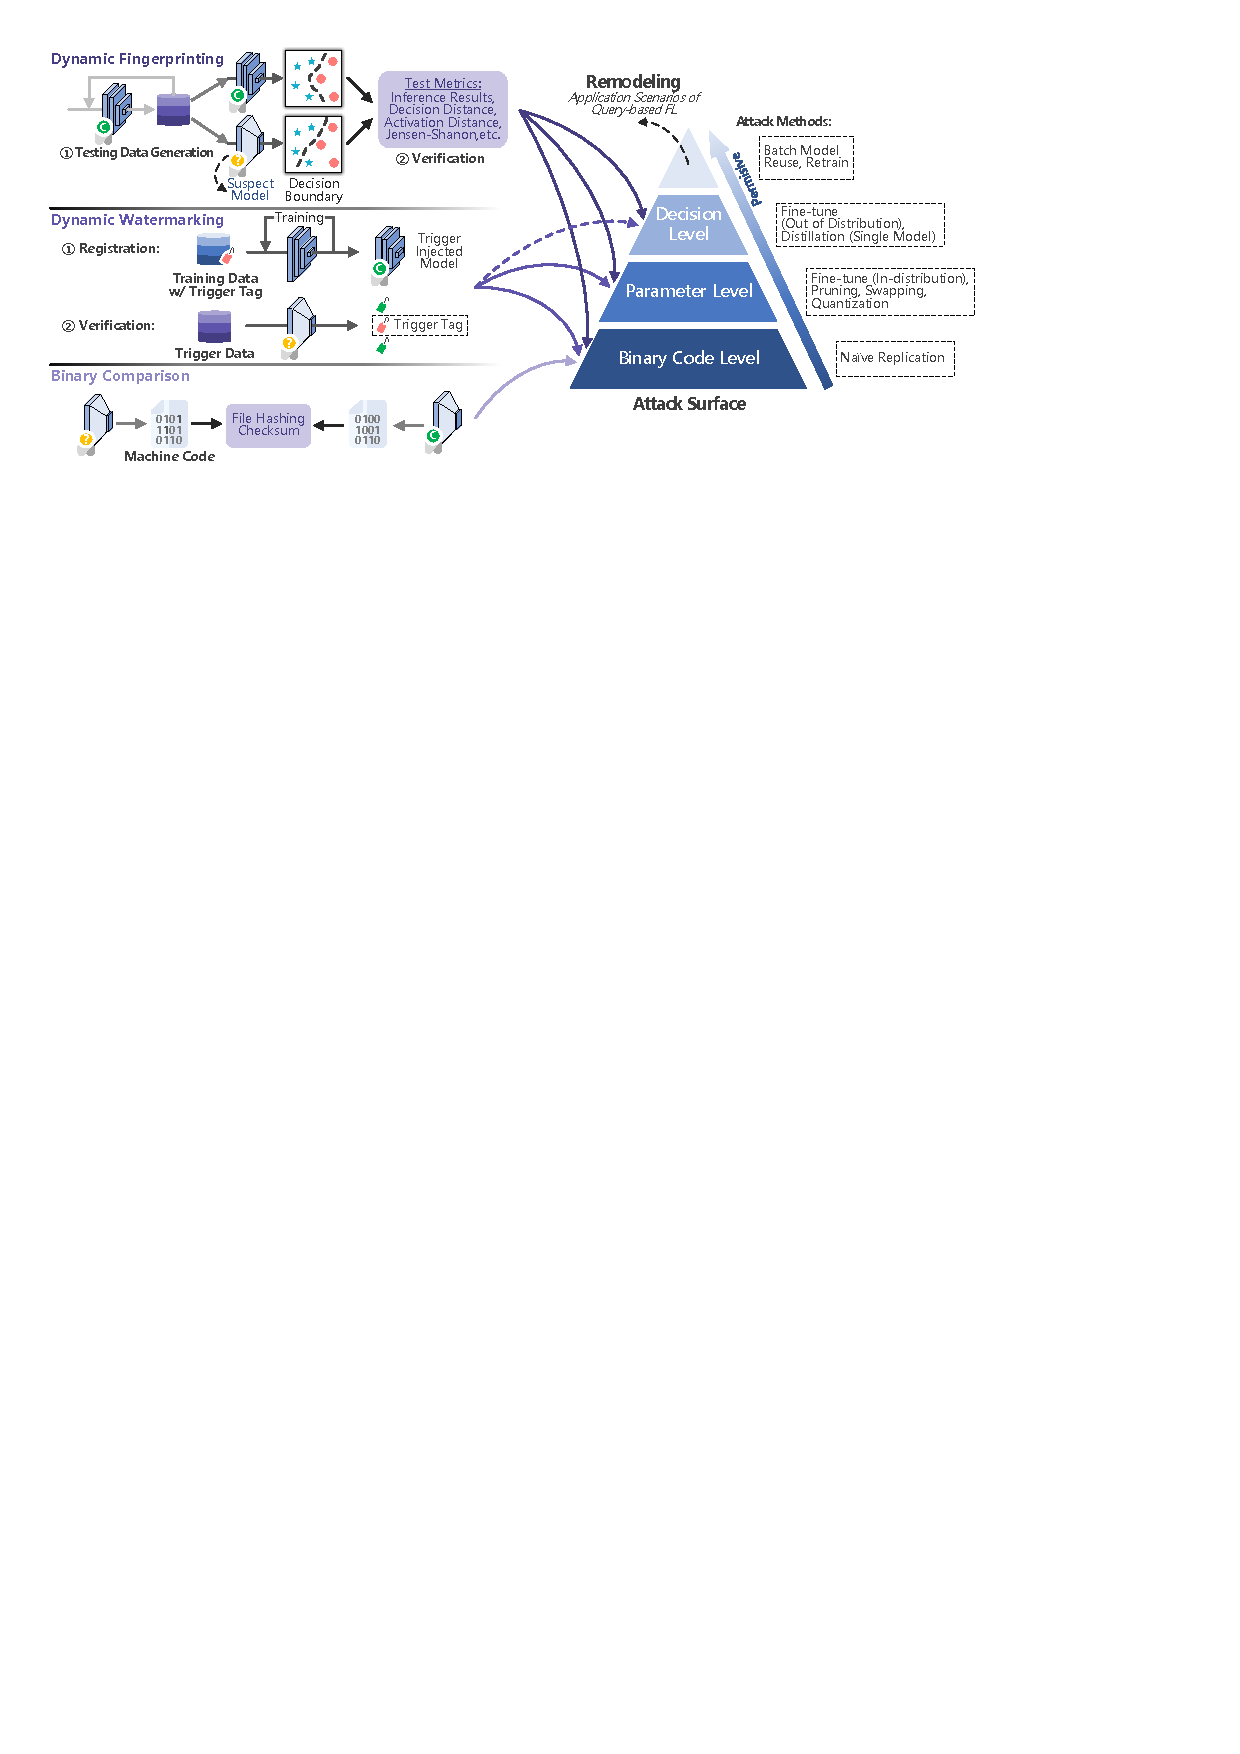
\includegraphics[width=\linewidth]{fig/ip_protection.pdf}
  \caption{Overview of DNNs IP protection methods.}
  \label{fig:ip}
\end{figure*}

First, it is helpful to consider the following requirements for model protection in the context of query-based FL:
\begin{itemize}
  \item \textbf{Non-invasive}. Any attempt to invasively embed backdoors into the weights and architectures of models is likely to result in changes to their functionalities and could lead to unexpected failures after deployment~\cite{chen2022copy}. 
  Meanwhile, these backdoors can be exploited by attackers to manipulate the model's predictions~\cite{li2022untargeted}.
  Accordingly, it is more recommend leaving the decision of adding invasive protection to the users instead of forcing it through platforms.
  
  \item \textbf{Compatible}. %模型未知
  Due to the model agnostic nature of query-based FL, relying on protection mechanisms that are specific to certain model structures and formats will limit the applicability of the platform.
  For instance, the passport layer~\cite{zhang2020passport} is built upon the normalization layer and requires joint training with the target model for ownership verification.
  However, in practice, both the normalization layer and whitebox access to the model may be unavailable.
  Therefore, considering the compatibility of model protection mechanisms is essential to ensure wide support for model sharing in query-based FL.

  \item \textbf{Permissive}. % 不对任何行为都检测
  As mentioned earlier, it is not essential to identify and address every instance of plagiarism in query-based FL. 
  On the contrary, we encourage platform users to engage in model mining and reusing. 
  Therefore, model protection methods should be permissive enough to allow for model reusing while still identifying the less creative effort operations that result in minimal or no change to the model's functionality, such as naive replication, quantization, pruning, and invariant neural swapping.
  Note that the presence of sufficient human creative effort is an important criterion for determining the copyrightability of a computer-generated work~\cite{national1979final}.
  The consideration of copyrightability can serve as a guiding principle in determining the scope of model protection in query-based FL.

  \item \textbf{Large-scale cost-effective}.
  Unlike traditional FL, where the size of training networks in each round is fixed, the size of a query-based FL platform is continuously expandable. 
  Therefore, it is undesirable if the potential conflicts~\cite{li2023fedipr}, required bit-length, and deployment cost~\cite{uchida2017embedding, darvish2019deepsigns} of model protection solutions such as watermarking and fingerprinting increase with the platform size.
  This suggests that solutions that require modifying optimization goals and training or fine-tuning with trigger data to embed identity information into the target model should be excluded.

\end{itemize}

Recently, several model protection algorithms have been proposed to address the challenge of model protection in FL. 
Tekgul \textit{et al.}~\cite{tekgul2021waffle} propose WAFFLE that uses augmented Gaussian noisy images as a watermark set to determine the ownership of the global model. 
However, this method is invasive and incurs high costs due to multiple rounds of training.
To ensure reliable watermarking for FL participants, FedIPR~\cite{li2023fedipr} embeds different watermarks into models of different participants through training with additional trigger samples and a modified optimization goal.
But this method is designed for model verification on the client-side, so it is independent to the model management in FL platforms.
FedTracker~\cite{shao2022fedtracker} embeds personalized local fingerprints into the Batch Normalization (BN) layer to enable traceability of model leakers.
One limitation of FedTracker is that its fingerprinting strategies are not compatible with other DNNs that do not use BN or do not provide whitebox access.
These examples highlight the incompatibility between the IP protection methods designed for traditional FL and the requirements of the query-based FL scenario, which have different protection goals and targets.

Based on the above observation and the taxonomy of deep IP protection~\cite{peng2022intellectual, sun2023deep}, \textbf{dynamic fingerprinting strategies with blackbox verification support} are considered suitable model protection methods for query-based FL.
These methods aim to approximate the similarities between the decision boundaries of different models by evaluating the value of a well-tailored testing metric on a self-constructed testing set.
A typical example is DeepJudge~\cite{chen2022copy}, which employs an ensemble of multi-level (Property, Neuron, Layer) testing metrics to achieve confident and robust plagiarism identification. 
The verification process of DeepJudge can be evaluated in a blackbox setting by calculating distances based on model predictions.
However, the generation of testing set in DeepJudge requires whitebox access to the suspect models in order to calculate adversarial samples, which may be unreachable if the suspect models are in binary format.

Another example is Zest~\cite{jia2022zest}, which randomly samples several training images and then applies super-pixel and segmentation techniques to construct the testing set.
However, this testing samples generation method is limited to images and may expose private training data.
A compromise approach is to seek non-sensitive or desensitized testing set from users when they upload their models.
Inspired by DeepJudge, we can develop an ensemble of multi-level testing strategies for query-based FL.
In the first step, we can compare the hash codes (e.g., MD5, SHA-256) of the raw model weights or its binary execution to rapidly filter out cases of naive replication plagiarism.
Then, in the second step, we can filter out cases of quantization or invariant neural swapping plagiarism by comparing the distance in predictions obtained from an out-of-distribution dataset.
In addition, we can further evaluate the similarities between models using testing-based approaches such as DeepJudge and Zest, which can detect cases of pruning and direct KD plagiarism.
Furthermore, if the workflow information is supports it, we can swiftly eliminate batch model reusing from being suspected of plagiarism.
To enhance understanding, we present an overview of the typical methods used for protecting IP of DNNs in Fig.~\ref{fig:ip}.

In summary, finding a balance between model protection and platform openness is indeed a challenge.
It is crucial to carefully consider the trade-offs and explore alternative approaches that can provide a reasonable level of model protection without excessively compromising the openness and usability of query-based FL platforms.



\section{Decentralization and Monetization in Contract-based FL} %%%%%%%%%%%%%%%%%%%%%%%%%%%%%%%%%%%%%%%%%%%%%%%%%%%%%%%%
\label{apdx:decentral}
Parallel to contract-based FL, several efforts are underway to build decentralized AI platforms through Web3-based techniques~\cite{guo2023blockchain}. 
For instance, Blythman \textit{et al.} proposed decentralized AI Hubs~\cite{blythman2022decentralized}, empowered by DAOs (e.g., IPFS~\cite{benet2014ipfs}, Ocean~\cite{mcconaghy2022ocean}, OpenMined), to run ML activities in a trustless setting.
Wickstr{\"o}m \textit{et al.}~\cite{wickstrom2022decentralizing} propose the concept of AI market which builds a ML analysis network for IoT devices based on Ethereum.
Similar to DMoE, Bittensor~\cite{steeves2022incentivizing} encapsulates neural network models as services and rewards peers contributing information-theoretic value to the system with TAO coins. 
Remote peers can be reused, for example, in the form of a MoE, or they can be pipelined to a new service.

The advantages of these blockchain-based systems are that transactions are transparent and workers can easily be incentivized.
Therefore, it is a solution when it is challenging to establish a trust relationship between platform users. 
However, if available, we can replace these DAOs' infrastructural components with a trusted crowdsourcing platform.
Like Amazon Mechanical Turk, the incentivized mechanisms is no nessary for contract-based FL platforms as the rewards are set by employers in contract.
While many studies consider Shapley value to evaluate the contribution of clients in FL systems~\cite{zhan2021survey}, we emphasize that a third-party evaluation can also be conducted in a crowdsourcing manner.
Similarly, as the model community in query-based FL, contract platforms can further provide IP protection services to users (ref. \ddag\ref{apdx:how2protect}). 
Dynamic fingerprints of models can be recorded and used for plagiarism detection.
Three kinds of interests should be considered: 1) Interest of employers, to prevent the information leakage of task configurations; 2) Interest of workers, requiring fair evaluation of labor; 3) Interest of the public, to curb the infringement of privacy.
However, this is not only a challenge from a technical perspective but also necessitates corresponding legislative oversight to provide guidelines to standardize this kind of AI marketplace commercialization.
We believe that a comprehensive regulatory framework is essential to ensure data privacy, and establish fair practices in the evolving landscape of open FL platforms.

\bibliographystyle{IEEEtran}
\bibliography{IEEEabrv,REF}

\vfill

\end{document}

\endinput